% Chapter 5
% add following line for typesetting from subfiles
% !TeX root = ../uet_thesis.tex
% !TeX root = ../uet_thesis.bbl
% !TeX root = ../references.bib
\chapter{Performance Optimization} % Write in your own chapter title
\label{Chapter5}
\lhead{Chapter 5. \emph{Performance Optimization}} % Write in your own chapter title to set the page header
%\section{Introduction}


%5)	Implementation and performance evaluation (Hardware + Error Probability)
%i)	Transmitter
%ii)	Receiver
%iii)	Practical results: P_e Vs Brightness Index
%iv)	Maximization Problem

The performance of proposed VR-MPPM codes depends upon several factors like brightness resolution, brightness index and channel conditions. The brightness resolution of VR-MPPM has a direct relation with codeword size. Therefore for better dimming control it is desired that the codeword size should be as large as possible. Information carrying capacity also increases with larger codewords. However there are certain constraints that degrade the line code performance if the codeword size is increased arbitrarily. Numerical performance evaluation results are provided for optimal choice of the symbol codeword size. System design parameters and constraints are formulated as an optimization problem to balance the underlying tradeoffs between brightness resolution and the successful data transmission. 

\section{Effect of Brightness Index and Brightness Resolution on Data Rate}

%As stated above before the information carrying capacity of the proposed codes is affected by the selection of the codeword. A larger code size ensures more brightness levels and better information carrying capacity per symbol frame. 

In this section the effectiveness of proposed VR-MPPM in meeting the desired objectives is observed. The code performance is evaluated numerically for $1 \leq n \leq64$. 

The coderate changes when brightness index is altered. It can be seen that coderate is minimum for $r=1$ and $r=n-1$. The former case is the simple pulse position modulation encoding that provides effective code rate of $\lfloor \frac{1}{n} \log_2 \binom{n}{1} \rfloor$ while the later is the inverted pulse position modulation. Coderate is same as that of PPM however the light source is operated at maximum brightness level. Maximum data rate is achieved when brightness index is $0.50$ i.e. $r=\frac{n}{2}$, providing effective coderate value of $\lfloor \frac{1}{n} \log_2 \binom{n}{n/2} \rfloor$.  The relationship of the two extreme parameters with frame size is plotted in figure \ref{fig:coderate_limits}. It can be observed from the graph that maximum coderate approaches unity for large $n$. On the other hand coderate decreases for lower brightness indices (near $r=1$) when frame size is increased.

The $50\%$ brightness index VR-MPPM line coding may find applications in other communication systems as well. In this case the VR-MPPM codes ensures $50\%$ duty cycle as the number of zeroes and ones is always equal in a codeword. It provides DC null and code transparency with bipolar-NRZ pulses. The maximum number of consecutive ones or zero's remains under $2(n-1)$ in worst case scenario. The available coderate is double as compared to Manchester or phase encoding.

\begin{figure}[h]
	\centering
	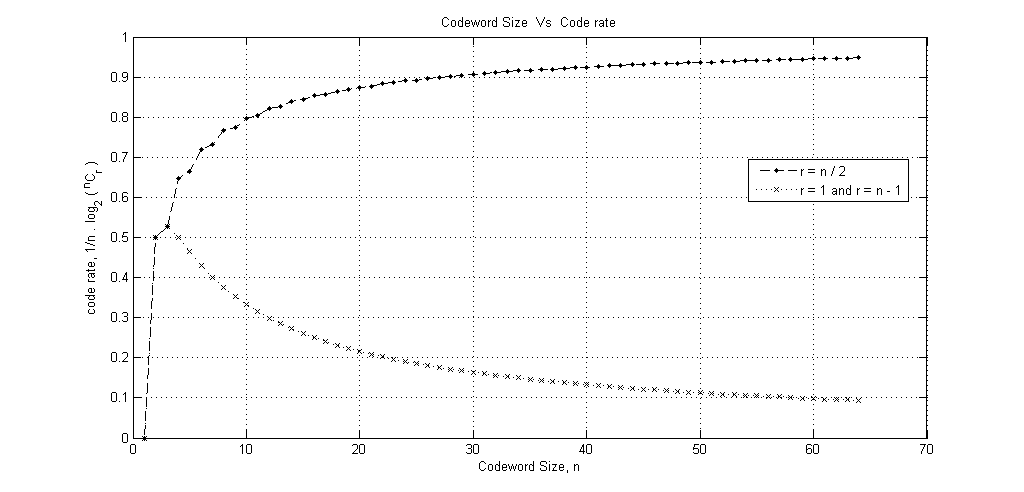
\includegraphics[width=\textwidth]{./Figures/max_min_coderate.png}
	\caption[Coderate limits imposed by $n$]{Upper and lower limits on coderate as function of frame size, n}
	\label{fig:coderate_limits}
\end{figure}

One more interesting result is the relationship between data transmission rate and the brightness index. The graph in figure \ref{fig:coderate_brightness} depicts the variations in coderate at different frame size $n$, where $n \in \{8, 16, 32, 64 \}$. The curve for fixed $n$ takes bell shape. Its the direct result of combinatorial relationship between frame size and brightness index, stated as $\binom{n}{r}=\binom{n}{n-r}$. The graph shows that the datarate is maximum in the middle of the curve where brightness index is $50\%$. The curves for different $n$ are farther apart from each other at this point which shows that the increased frame size has more pronounced increase in coderate when $r=\frac{n}{2}$ 


\begin{figure}[h]
	\centering
	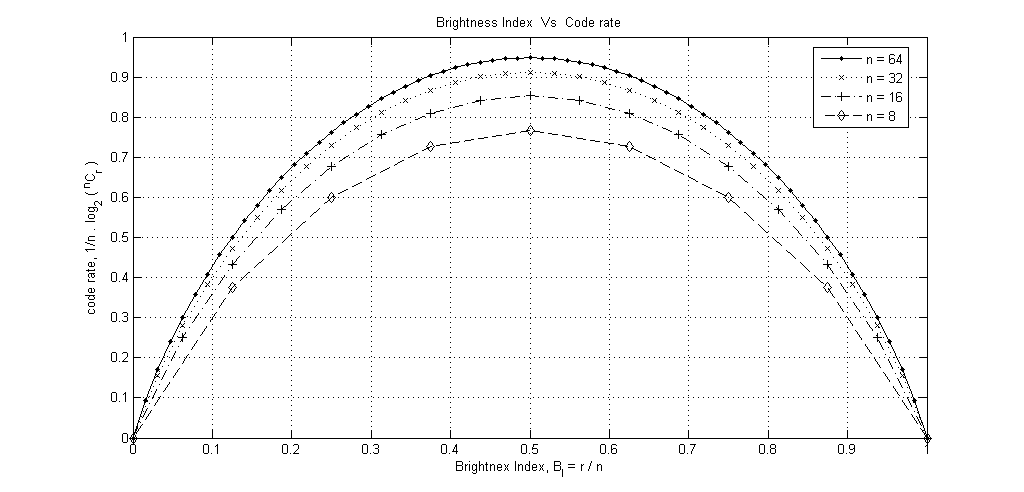
\includegraphics[width=\textwidth]{./Figures/coderate_brightness.png}
	\caption{Dependence of code-rate on brightness index}
	\label{fig:coderate_brightness}
\end{figure}


\section{Optimal Frame Size And Channel Conditions}
 It has been discussed earlier that both the brightness resolution and information carrying capacity of the VR-MPPM code improves when frame size is increased. However the symbol error probability also increases with the number of slots per frame, $n$. Therefore the frame size can not be increased arbitrarily. The effect can be observed by the relationship between single bit error probability, $p_e$ and the symbol decoding error probability, $p_s$ given be equation \ref{eq:error_probability}:

\begin{equation}
p_s=\left[1-(1-p_e)^n \right]
\label{eq:error_probability}
\end{equation}

The probability of correctly detection of a symbol given be the equation \ref{eq:correction_probability}, decreases with increasing frame size $n$. The parameter $p_{s,corr}$ is plotted for two different values of single bit error probability $p_e$ in figure \ref{fig:symbol_error}

\begin{equation}
 p_{s,corr}=\bar{p}_s=(1-p_e)
\label{eq:correction_probability}
\end{equation}

\begin{figure}[h]
	\centering
	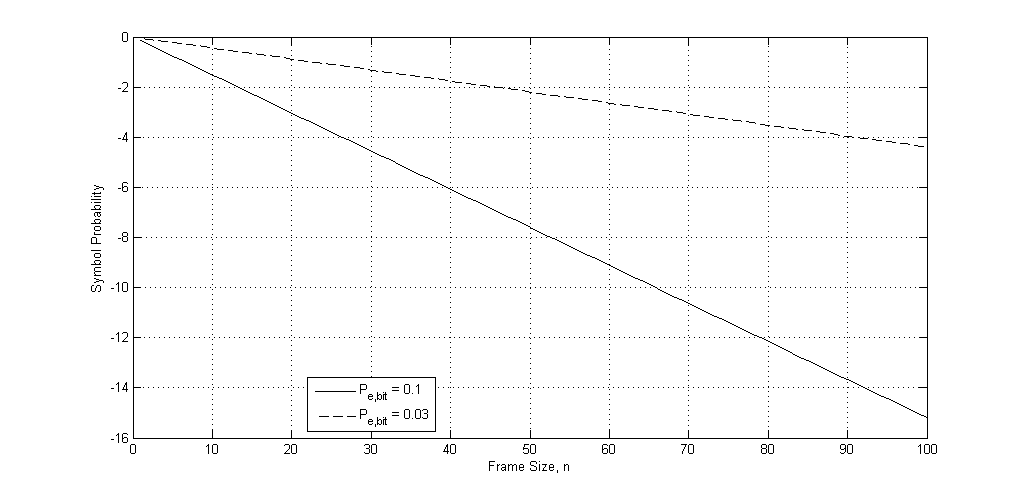
\includegraphics[width=\textwidth]{./Figures/SymbolVsn.png}
	\caption[Symbol correctly decoding probablity]{Symbol correctly detection probability as a function of frame size}
	\label{fig:symbol_error}
\end{figure}

It is aimed that the encoding scheme should provide maxim datarate and maximum control over brightness levels with minimum symbol error count.These contradictory requirements point towards finding an optimal size of the codeword such that the brightness resolution and symbol correctly detection probability $p_{s,corr}$ are maximum possible. It leads to the evaluation of the optimization problem defined by equation \ref{eq:objective_function}. The objective function is plotted for two bit error probabilities in figure \ref{fig:objective_function}. Peak values in the graph indicate the optimal frame size for a given value of bit error probability $p_e$

\begin{figure}
	\centering
	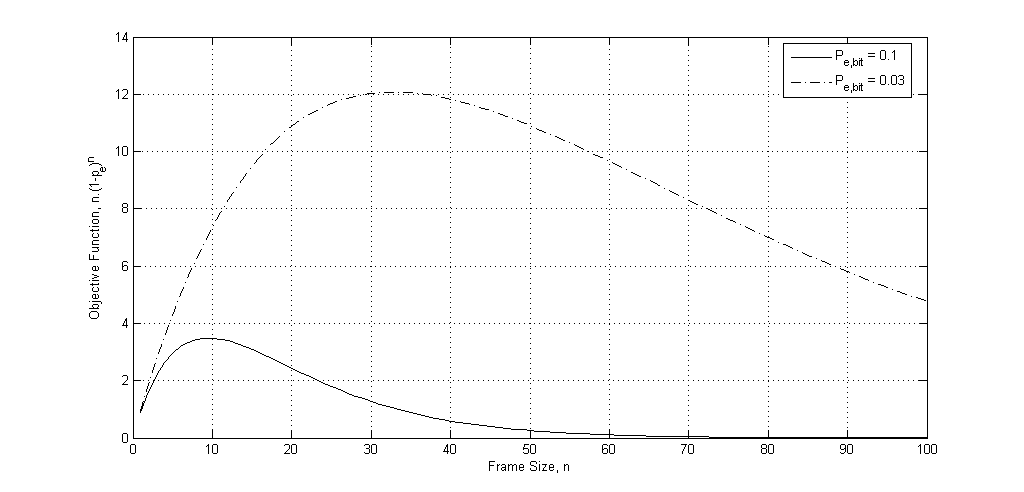
\includegraphics[width=\textwidth]{./Figures/ObjectiveFunction.png}
	\caption{Encoder frame size objective function}
	\label{fig:objective_function}
\end{figure}

\begin{equation}
\begin{array}{cc}
\mathbf{maximize}& f(n)=n(1-p_e)^n \\
\mathbf{subject~to}& 0<n, 0 \leq p_e \leq 1
\end{array}
\label{eq:objective_function}
\end{equation}

The value of $n$ in equation \ref{eq:objective_function} can be relaxed to be a positive integer as it defines the number of bits in a codeword. To check for global optimality of the solution given by objective function, its second derivative is evaluated as

\begin{equation}
f''=(\bar{p}_e)^n \ln (\bar{p}_{s,corr})(n \ln \bar{p_e} + 2)
\label{eq:second_d}
\end{equation}

Where $\bar{p}_e=(1-p_e)$ in equation \ref{eq:second_d}. The objective function based upon \ref{eq:second_d} is identified as

\begin{equation}
    f(n) = \left\{\begin{array}{cccc}
    concave & as~ f''(n) \leq 0  & for & \frac{2}{|\ln (1-p_e)|} \geq n \\
    convex & as~ f''(n) \geq 0  & for & \frac{2}{|\ln (1-p_e)|} \leq n
\end{array}   \right..
\label{eq:concavity}
\end{equation}

The solution for equation \ref{eq:objective_function} finally evaluates as

\begin{equation}
\psi (n) = \frac{1}{n}
\end{equation}

The optimality function $\psi(n)$ is plotted as a function of channel bit transitional probability $p_e$ in figure \ref{fig:optimal_function}


\begin{figure}{htbp}
	\centering
	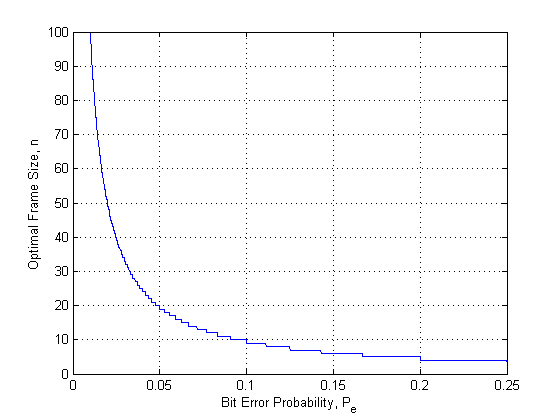
\includegraphics[width=\textwidth]{./Figures/OptimalFunction.png}
	\caption{Optimal value of frame size Vs Bit transition probability}
	\label{fig:optimal_function}
\end{figure}
%=======================================
The curve provides the optimal number of bits per codeword for a given channel bit transition probability $P_e$ on horizontal axis.

%\section{Hardware Implementation}
%Effectiveness of the proposed solution was shown by hardware implementation. We did hardware test on two platforms. The first implementation uses the RS232 protocol to drive the light source. The second implementation is the FPGA implementation using Digilent Nexys-2 FPGA board \cite{nexys2}.
%
%\section{RS-232 Based Implementation}
%First one implements the variable rate pulse position modulation (VR-MPPM) using byte transmission in UART communication. A USB to UART cable was used to interface the transmitter and receive modules to the computer. The converter cable used Texas Instruments chip TUSB3410\cite{TUSB3410} that supports speeds upto 921600 baud. The transmitter consists of 84 high brightness white LEDs mounted in grid form of $6\times 14$ LED. 14 LED are connected in parallel in a string. Three such strings are connected in series connection to form a $3\times 14$ LED bank. That means a bank of LEDs can be lighted from a 12V DC wall adapter. Two such banks are connected in parallel in the transmitter shown in figure \ref{fig:tx_hardware}. Texas Instruments' half-bridge bipolar switching integrated circuit UC2950T \cite{UC2950} is used as power driver.
%
%\begin{figure}[hbtp]
%\centering
%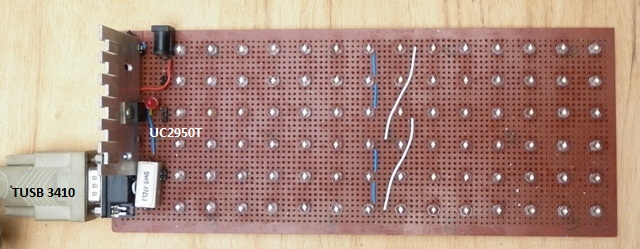
\includegraphics[angle=0,width=0.9\textwidth]{./Figures/Transmitter.jpg}
%\caption[VLC transmitter hardware]{VLC transmitter light consists of 84 High brightness White light LED}
% \label{fig:tx_hardware}
%\end{figure}
%
%The receiver module is built around toshiba TORX173 \cite{TORX173} optical fiber receiver for digital audio. This particular module is easily available in the market. It provides clean TTL electrical output signal  that is stabilized over wide range of optical signal power level. This makes the interfacing with TUSB3410 \cite{TUSB3410}, USB to UART converter, hassle free. The optical receiver module supports data rates upto 6MHz that covers full range of the converter and LED driver chips. Receiver module is shown in figure \ref{fig:rx_hardware}. 
%
%\begin{figure}[hbtp]
%\centering
%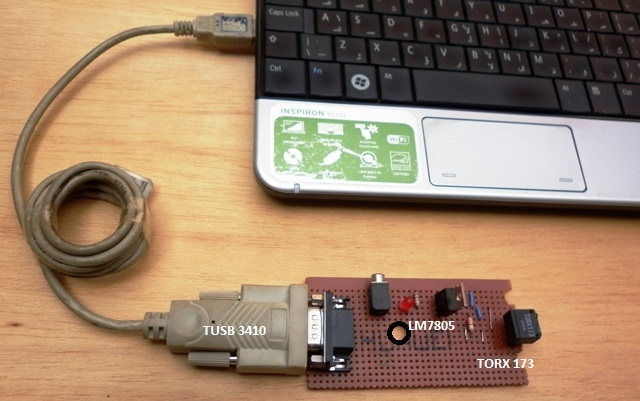
\includegraphics[angle=0,width=0.75\textwidth]{./Figures/Receiver_v2.jpg}
%\caption[VLC receiver hardware]{VLC receiver built around Toshiba TORX173 integrated optical receiver module}
%\label{fig:rx_hardware}
%\end{figure}
%
%%The hardware setup is used to evaluate the symbol error probability at different brightness indices. The graph in figure \ref{fig:evaluation1_hardware} shows the relationship. It is observed that minimum symbol error rate is achieved at around $0.5$ brightness index. Beyond that point on either side error probability is higher due to saturation of the receiver owing to unbalanced one-zero stream.
%%\begin{figure}
%%	\centering
%%	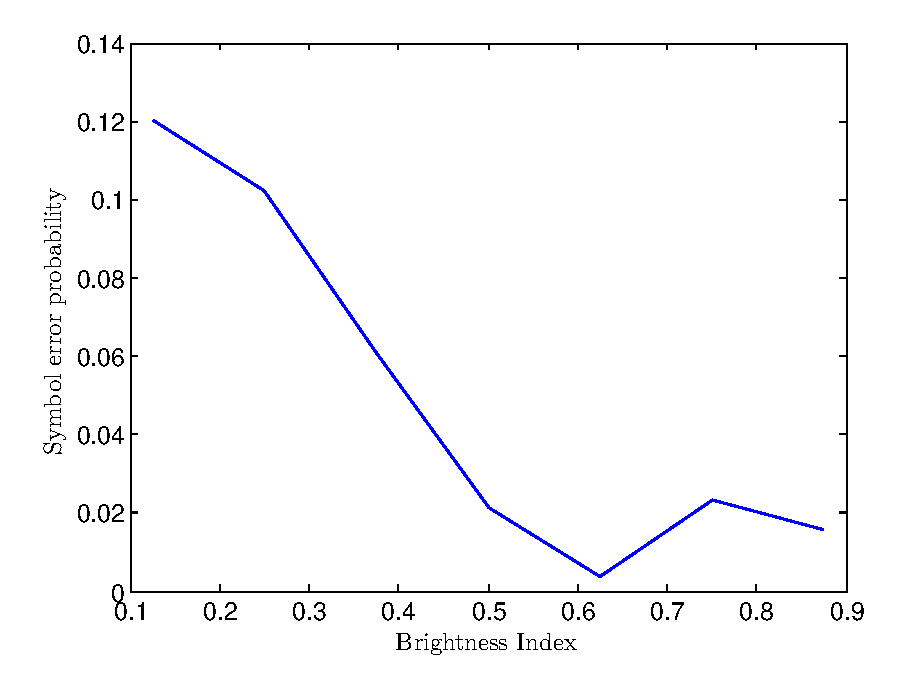
\includegraphics[width=\textwidth]{./Figures/experiment_brightness}
%%	\caption[Effect of brightness index on symbol error rate]{Practical evaluation: Effect of brightness index on symbol error rate}
%%	\label{fig:evaluation1_hardware}
%%\end{figure}
%
%
%\section{FPGA implementation on Xilinx Spartan-3 board}
%
%Although UART based implementation is easier to set up as this protocol has been one of the most popular data interfacing schemes and is already supported by a lot of devices however brightness control in this implementation is limited. The start and stop bits inserted by the protocol introduce extra time slots whose value can not changed according to the desired brightness level.
%
%To test the effectiveness of the proposed solution we implemented the VR-MPPM scheme using FPGAs. This implementation was used to evaluate the data rate and error performance of the proposed codes over more wider range of frame size and brightness indices. This implementation provides better control over brightness level along with faster data transmission as overhead bits do not effect the output stream. The prototype is set up in loop-back fashion with both the encoder and the decoder implemented on Nexys-2 \cite{nexys2} board from digilent. This board hosts Xilinx Spartan 3E-500 FG320 FPGA chip.  Verilog Hardware Description Language (HDL) was used to implement the logic. Hardware is described at behavioural level therefore no significant difference is there between the earlier listed algorithms \ref{algo:Encoder} \ref{algo:Decoder}  and the Verilog HDL code.
%
%%\begin{figure}[hbtp]
%%\centering
%%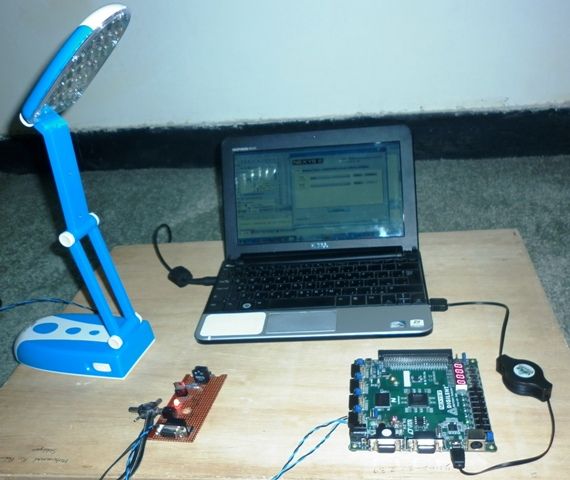
\includegraphics[angle=0,width=0.75\textwidth]{./Figures/Lamp_Off.jpg}
%%%\caption{VLC setup with Nexys-2 Development Board}
%%\label{fig:VLCNexys2On}
%%\end{figure}
%%
%%
%%\begin{figure}[hbtp]
%%\centering
%%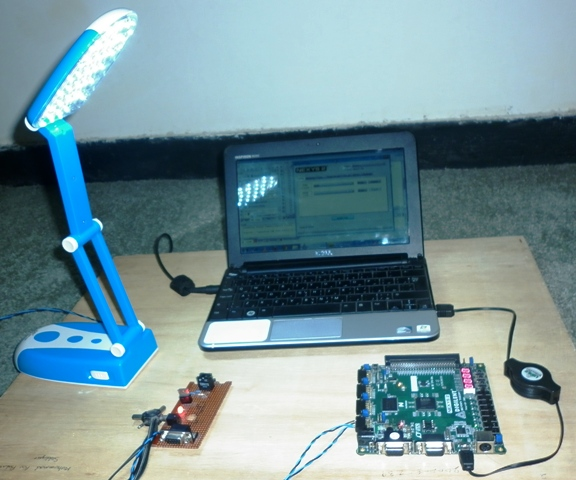
\includegraphics[angle=0,width=0.75\textwidth]{./Figures/Lamp_On.jpg}
%%\caption{VLC setup with Nexys-2 Development Board}
%%\label{fig:VLCNexys2Off}
%%\end{figure}
%
%
%
%\begin{figure}[hbtp]
%\centering
%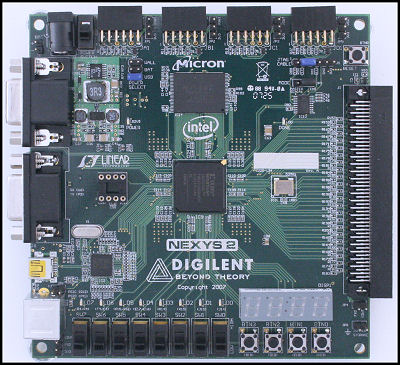
\includegraphics[angle=0,width=0.75\textwidth]{./Figures/NEXYS2_400.jpg}
%\caption{Nexys-2 Development Board}
%\label{fig:nexy2}
%\end{figure}
%
%\subsection{Encoder Module}
%The encoder implements the algorithm discussed in Chapter-\ref{Chapter3} algorithm:\ref{algo:Encoder}. It requires 'n' clock cycles to convert the input symbol to n-bit codeword sequentially. The combinatorial function required by the encoder $binom{n}{r}$ is implemented using the lookup table. Same lookup table is used by the decoder as well. This table is implemented in a separate module \textbf{nCrROM} as listed in appendix \ref{sec:nCrROM}. The encoder evaluates the most significant bit first and provides encoded data both in serial and parallel form. The $complete$ signal is asserted after encoding process is complete. Parallel output can be read correctly after this signal is set. Encoding process is started after detecting a high level on $start$ input at positive clock edge. Signal $m$ is the input signal that is coded with bits defined by $frameSize$. The output codewords is generated with $r$ pulses slots.
%\begin{figure}[h]
%	\centering
%%	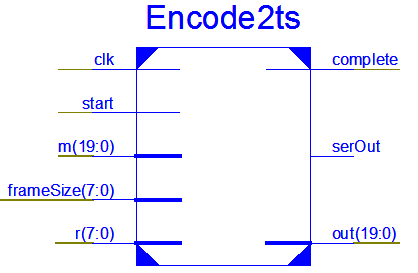
\includegraphics{./Figures/Encode2ts.png}
%	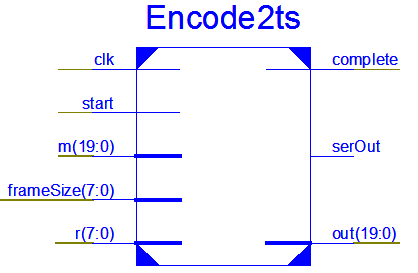
\includegraphics[width=.5\textwidth]{./Figures/Encode2ts.png}
%	\caption{VR-MPPM encoder module}
%	\label{fig:Encode2ts}
%\end{figure}
%\subsection{Decoder Module}
%The decoder is implemented using algorithm \ref{algo:Decoder}. Decoder, too, requires 'n' clock cycles to convert the n-bit input codeword back to the original symbol. It evaluates the most significant bit first. Therefore encoder and decoder module can work back to back with a serial link. The decoder can also take in the codeword as a parallel word. It is read in at positive clock edge after the signal $start$ is set. All other signals are same as described for the encoder.
%
%\begin{figure}[h]
%	\centering
%%	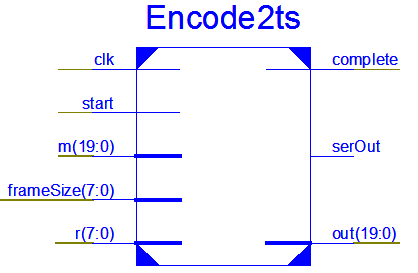
\includegraphics{./Figures/Encode2ts.png}
%	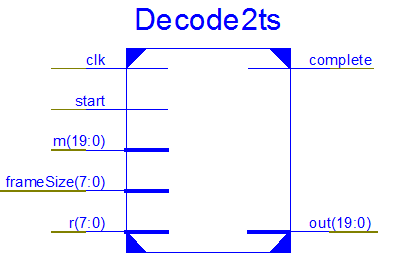
\includegraphics[width=.5\textwidth]{./Figures/Decode2ts.png}
%	\caption{VR-MPPM decoder module}
%	\label{fig:Decode2ts}
%\end{figure}
%
%\subsection{Parallel to Serial and Serial to Parallel Module}
%The functionality of this module is to transmit and receive the parallel data on an external serial link. Serial link in this case consisted of the visible light communication optical link. Because we needed to check the link performance for VR-MPPM at different frame sizes and brightness indices, serial data was sent on $serOut$ at positive clock edge and read in through $serIn$ on negative edge of the clock. The Nexys-2 boards's Pmod port JA1 was used to transmit and receives the data on serial link consisting of white light LED and TORX-173 optical receiver. The Verilog implementation is listed in appendix \ref{sec:p2p}
%\begin{figure}[h]
%	\centering
%	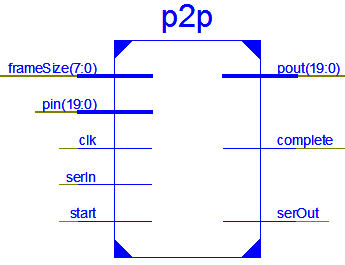
\includegraphics[width=.5\textwidth]{./Figures/p2p.png}
%	\caption{Serial link module}
%	\label{fig:p2p}
%\end{figure}
%
%\subsection{Encoded Parallel$\leftrightarrow$Serial Module}
%This is an upper level module that integrates the encoder, p2p and encoder module, thus completing the serial link with VR-MPPM encoded data. As encoder and decoder operate at very high nexys-2 board frequency, this module generates a slower clock frequency suitable for white LED operation. The input word $pin$ is first encoded using encoder module \ref{sec:Encode2ts}. When this conversion is complete it is sent over serial link using p2p module \ref{sec:p2p}. After parallel$\leftrightarrow$Serial complete signal is asserted the data is received in completely and is fed to the decoder module \ref{sec:Decode2ts}. This module's $complete$ signal is asserted after all the three stages have been completed.
%
%\begin{figure}[h]
%	\centering
%	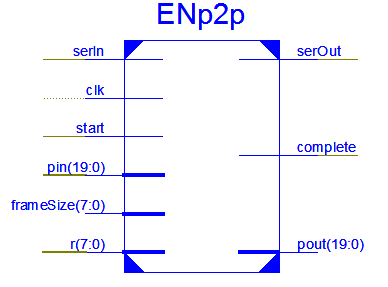
\includegraphics[width=.5\textwidth]{./Figures/ENp2p.png}
%	\caption{VR-MPPM encoded serial link module}
%	\label{fig:ENp2p}
%\end{figure}
%
%\subsection{Module for Scanning VLC Codes}
%The scan codes \ref{sec:scanCodes} module was implemented to check the error rate performance of the optical link by cycling through all possible symbols in cyclic form, for a particular selection of frame size and brightness index. This module keeps record of the error count by comparing the received and transmitted symbols.
%
%\begin{figure}
%	\centering
%	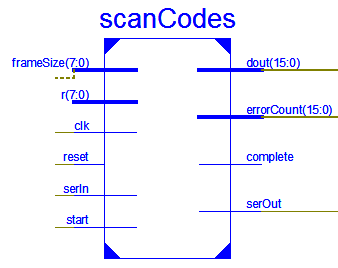
\includegraphics[width=.5\textwidth]{./Figures/scanCodes.png}
%	\caption[Module for generating scan symbols]{Generate VR-MPPM symbols for onboard evaluation of bit error rate}
%%	\caption{HDL block to generate, transmit and receive VR-MPPM symbols for onboard evaluation of bit error rate}
%	\label{fig:scanCodes}
%\end{figure}
%
%\subsection{VLC Module}
%VLC is the top level module. It defines the ports and signals of the Nexys-2 board that are used during actual functionality test. The user constraint file $toplevel.ucf$ \ref{sec:toplevel} defines the mapping of board ports to VLC module signals.
%
%
%%\begin{figure}[hbtp]
%%\centering
%%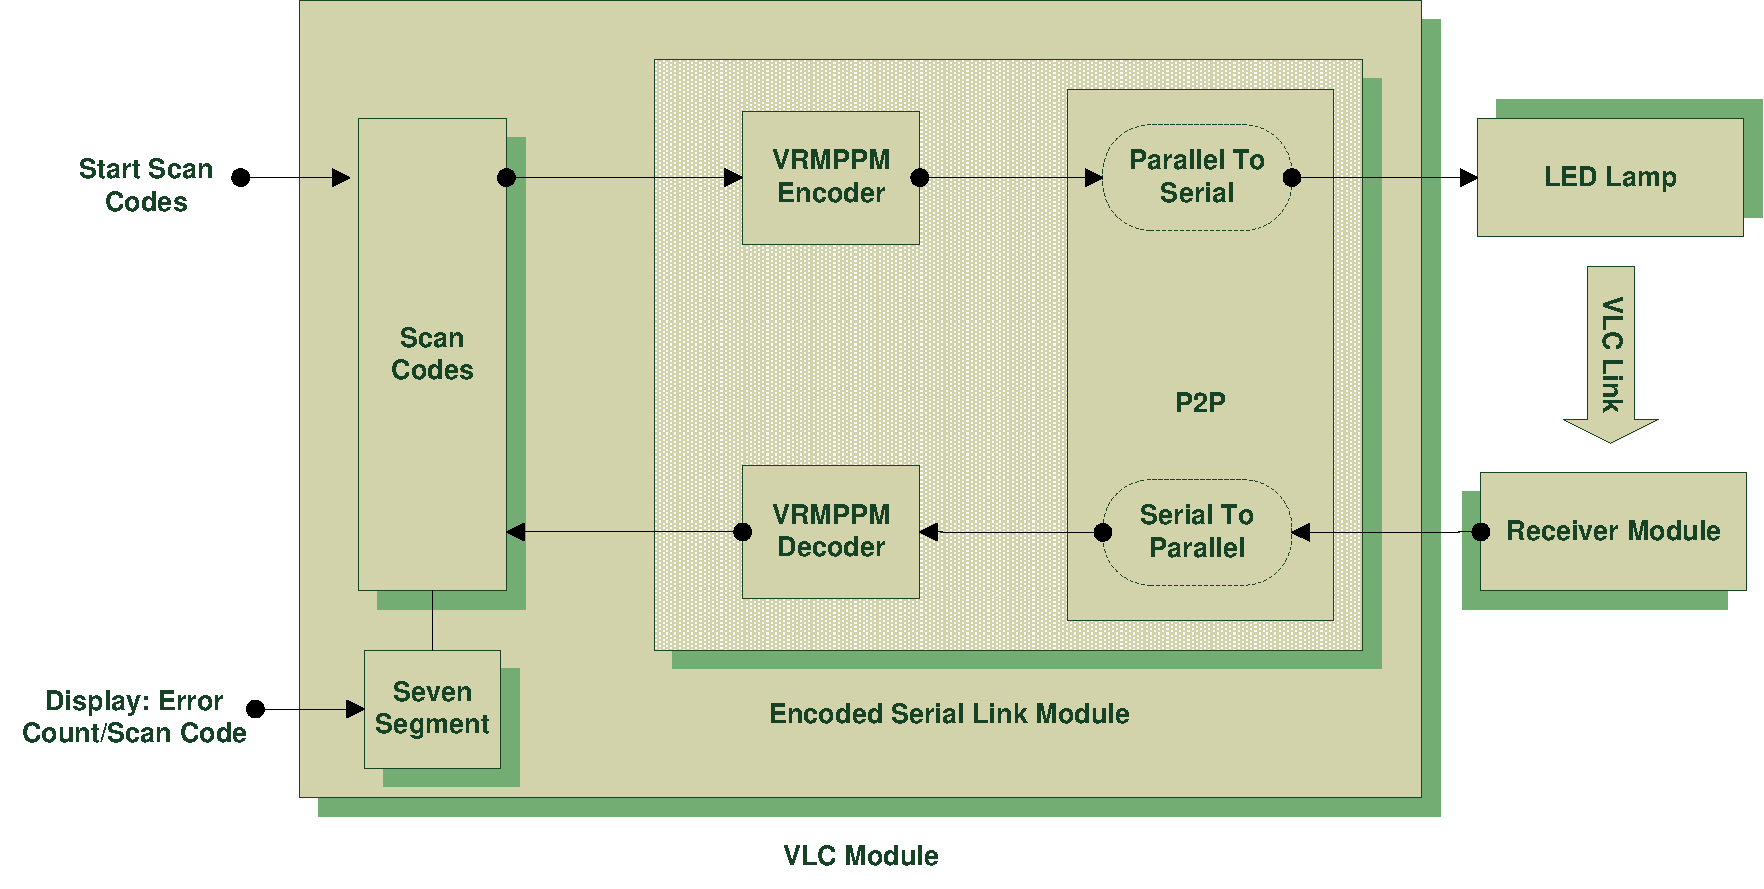
\includegraphics[angle=0,width=\textwidth]{./Figures/VLC_block_diagram}
%%\caption{FPGA Implementation Block Diagram}
%%\label{fig:FPGAblock}
%%\end{figure}
%
%%\subsection{User Constraints File}
%%The constriant file \ref{sec:toplevel} for Nexys-2 board defines the pins used for VLC module signals.
%
%\begin{figure}[h]
%	\centering
%	\includegraphics[width=.5\textwidth]{./Figures/vlc.png}
%	\caption[Toplevel VLC module]{HDL block diagram of top level module for serial link simulation}
%	\label{fig:vlc}
%\end{figure}
%
%\subsection{Clock Divider Module}
%The basic clock of Nexys-2 board runs at 50MHz. This frequency is much higher than the capability of commonly available white LEDs. Therefore it is requiered to slow down the actual transmitting frequency to within a few megahertz. The clock divider module \textbf{clkDiv} takes in the system clock signal and outputs a new clock that is slowed down by the count value defined by the input word $newDiv$.
%
%\begin{figure}[h]
%	\centering
%	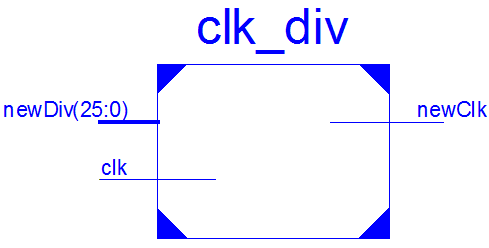
\includegraphics[width=.5\textwidth]{./Figures/clk_div.png}
%	\caption[]{Clock divider module}
%	\label{fig:clkDiv}
%\end{figure}
%
%
%\subsection{Seven Segment Driver Module} The Nexys-2 board houses a four digit seven segment display. This module drives the display to represent 16-bit word in hexadecimal format \ref{sec:LED_7seg}.
%
%\begin{figure}[h]
%	\centering
%	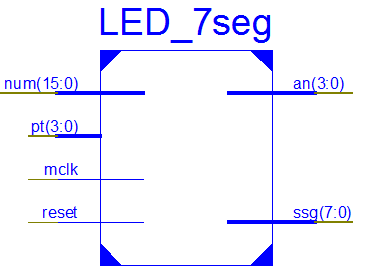
\includegraphics[width=.5\textwidth]{./Figures/LED_7seg.png}
%	\caption{7-segment drivier module to display 16-bit values }
%	\label{fig:LED_7seg}
%\end{figure}
%
%\section{Experimental Results}
%
%The performance of a VR-MPPM visible light link at different brightness indices was evaluated using a FPGA platform. Transmitter and Receiver module were implemented on Digilent's Nexys-2 board. The transmitter consisted of off the shelf white LEDs. The receiver was built around TORX173 optical receiver module from Toshiba. Receiver and transmitter were interfaced to the Nexys-2 board using two interface lines of the $JA$ pmod connector. Symbol error rate was observed for three different values of frame size by varying the brightness index in the available range. The results are represented in figure \ref{fig:fpgaExperiment}. It can be observed that code error performance degrades for larger frame size at fixed brightness index, as depicted by equation \ref{eq:error_probability}.
%
%\begin{figure}[h]
%	\centering
%	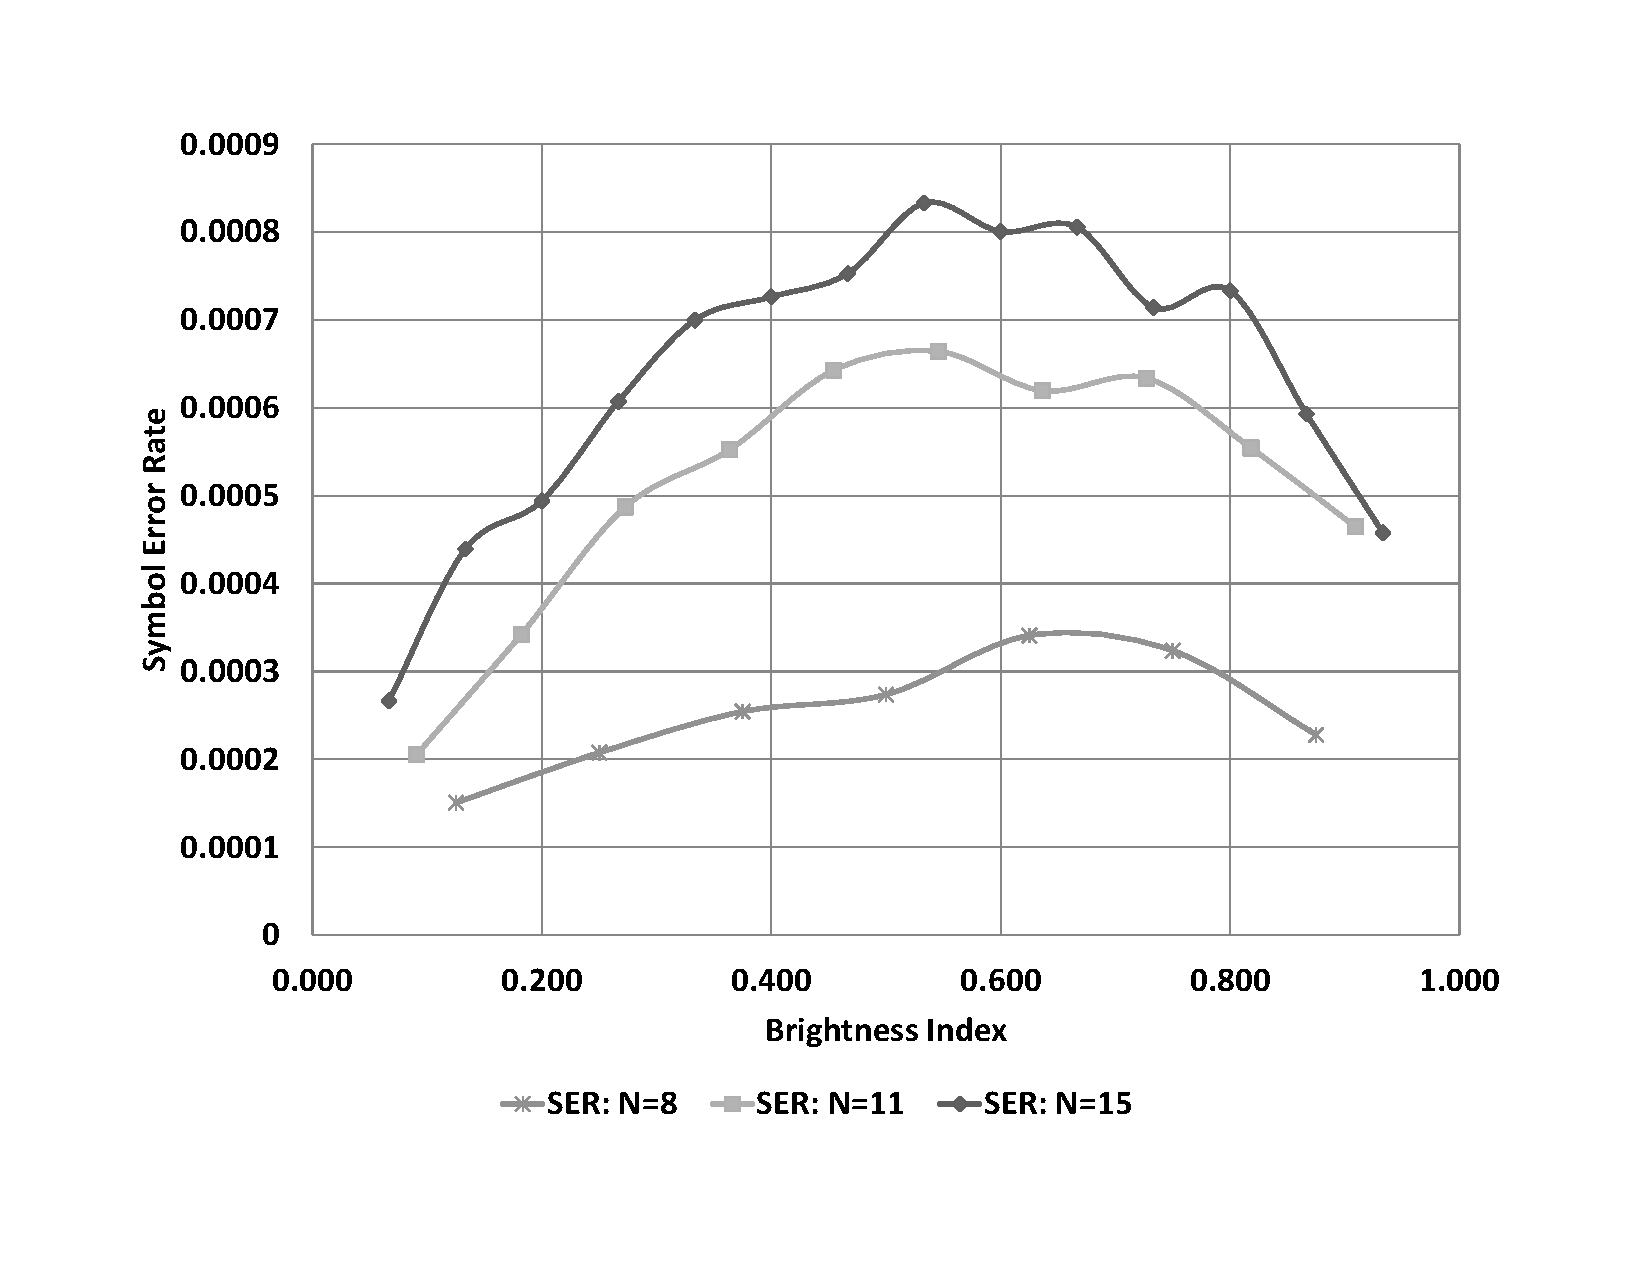
\includegraphics[width=\textwidth]{./Figures/Experiment}
%	\caption[Hardware Performance Evaluation]{Symbol error rate evaluation of VR-MPPM encoded symbols at different brigness indices. $n$ represents the frame size.}
%	\label{fig:fpgaExperiment}
%\end{figure}
%
%For a given frame size, the symbol error rate curve takes a bell shaped curve with maximum number of errors encountered around 50\% brightness. From discussion of the proposed VR-MPPM codes it is known that maximum bit transitions occur for 50\% brightness as shown in figure \ref{Fig:line_codes2}. There are more bandwidth constraints on a fast switching signal. That counts for the greater number of errors.
%
%The experimental results are also in close agreement to the MPPM channel modelling presented in \cite{hamkins2005multipulse}. 
%
%%
%%Let $p_0(y)$ denotes the conditional probability of decoding a bit as 'y' when a zero was transmitted and $p_1(y)$ is the probability of decoding 'y' when a one was transmitted. Suppose in a frame size consisting of 'n' time slots of which first 'r' time slots contain a one and last 'n-r' slots contain a zero. Considering the discrete memory less channel with hard detection, the probability of decoding error of a symbol 's' is given by:
%%
%%\[
%% P_{ser} = (probability~of~1\rightarrow 0~transition)^r \times  (probability~of~0\rightarrow 1~transition)^{n-r} 
%%\]
%%
%%Now there are a total of $2^n$ codewords possible with $n$ slots. We need to calculate the probability for $\binom{n}{r}$ symbols in group of total possible symbols. It provides with the probability of symbol decoding error with $r$ ones as
%%
%%\[
%% P_{ser,r} = \frac{1}{2^n} \binom{n}{r}(probability~of~1\rightarrow 0~transition)^r \times  (probability~of~0\rightarrow 1~transition)^{n-r} 
%%\]
%%
%%
%%\begin{equation}
%% P_{ser,r} = \frac{1}{2^n} \binom{n}{r} p_1^r(0) \times  p_0^{n-r}(1) 
%%\label{eq:ser2}
%%\end{equation}
%%
%%Equation \ref{eq:ser2} hints at a bell shaped curve for symbol error rate performance.
%
%
%
%\begin{figure}[h]
%\centering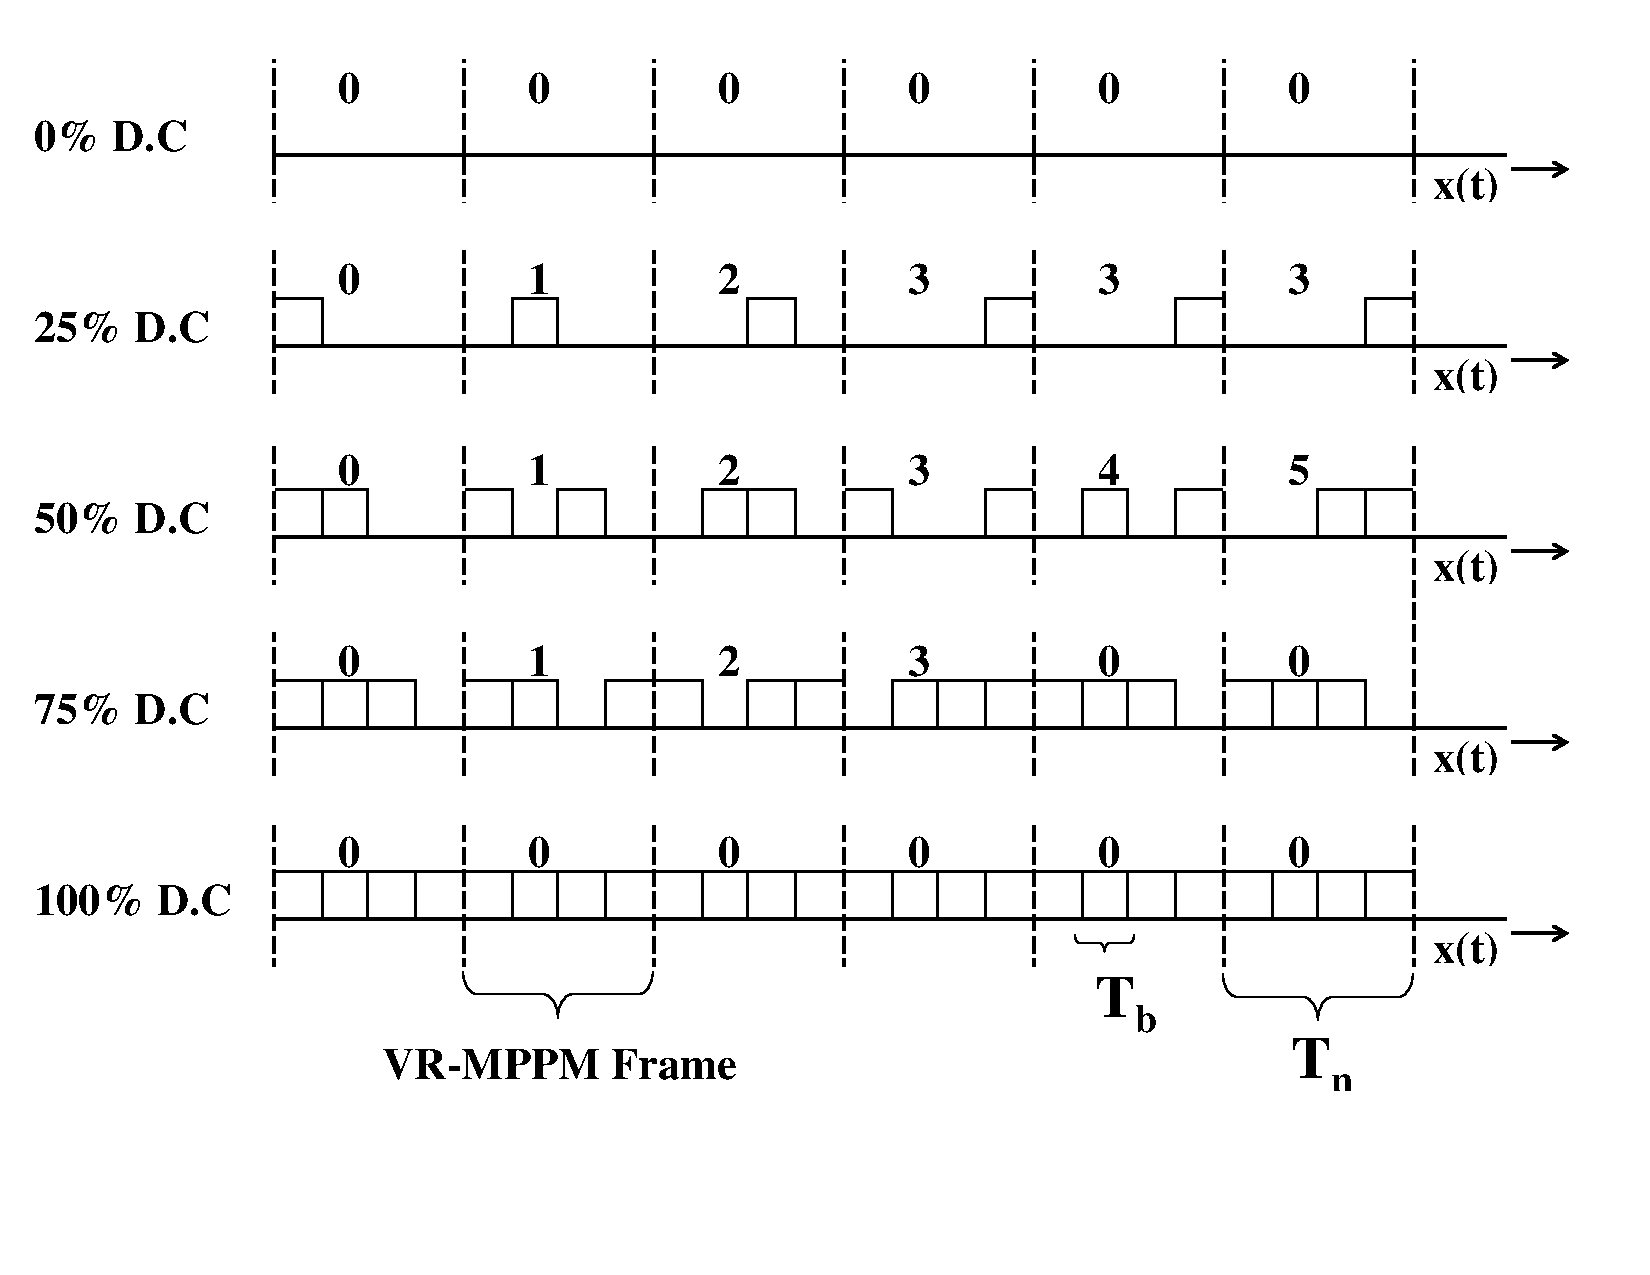
\includegraphics[width=\textwidth]{./Figures/line_code}
%\caption[VR-MPPM line waveforms]{VR-MPPM waveforms: Maximum transitions occur at 50\% brightness}
%\label{Fig:line_codes2}
%\end{figure}